
\section{External Forces and Moments}

In addition to gravity acting on a vehicle, other forces also act
on the satellite. For a 1U CubeSat, the gravity gradient over 10 cm is about
$0.24~\mu m/s^2$ using the EGM2008 model. Multiplying this 
acceleration by a $1~kg$ mass and applying a $10~cm$ moment arm yields
a moment of about $2.4 \times 10^{-8}~N-m$. Aerodynamic torques could
be as large as $1.5 \times 10^{-10}~N-m$ assuming the aerodynamic
center is 5~cm away from the center of mass. Typical magnetorquers operate
in the vicinity of $3.0 \times 10^{-6}~N-m$, assuming a current of $0.04~A$, an area of
$0.02~m^2$, 84 turns and a magnetic field of $40,000~nT$. Using
these calculations, magnetorquers are two orders of magnitude
larger than gravity torques and four orders of magnitude larger than
aerodynamic torques. It is important to keep these values in mind when
neglecting certain parameters
\cite{Radiation,AndersonD,Density_Model}.

\subsection{Solar Radiation Pressure}

Solar radiation pressure is relatively constant at 1 AU and thus is
simply given as $p_s=4.5e-6~Pa$. The force is then found to be just
the pressure multiplied by the frontal area of the satellite. The
torque, similar to the aerodynamic torque, is the force crossed with a
distance vector from the center of mass to the center of pressure of
solar radiation. The vector $\hat{s}$ is a unit vector denoting the
direction of the sun.
\begin{equation}
  \vec{F}_{SR} = p_s S \hat{s}
  \end{equation}
\begin{equation}
    \vec{M}_{SR} = {\bf S} \left( \vec{F}_{SR} \right) \vec{r}_{CG-CPs}
\end{equation}

\subsection{Propulsion Model}

In order for a vehicle to lift off to enter space, engineers must be
able to apply a force that is greater than the force acting on the
vehicle due to gravity and aerodynamics.  The applied force is known
as thrust. Thrust can be generated by the propulsion system of the
vehicle. Electric and chemical are two well-known methods to produce
thrust which take advantage of Newton’s third law of motion.

Electric Propulsion Systems typically use electric heating or electric
or magnetic fields to accelerate propellants (usually gases).  These
systems can be very fuel-efficient, however it does not generate
enough thrust. These engines are great for deep space exploration
where transit times can be very long and rapid maneuvers are not
required\cite{qp8}.

Chemical propulsion systems are  more effective in our
environment. These systems involve the use of chemical reactions to
release energy and accelerate gases to produce thrust. Chemical
propulsion is a broad category and can be subdivided into liquid
propulsion, solid propulsion, and hybrid propulsion.

Liquid propulsion systems can be further subdivided into either a
monopropellant (a single propellant fluid) or a bi-propellant (two
fluids, which includes fuel and an oxidizer). The simplest form of
fuel and oxidizer would be liquid hydrogen and liquid
oxygen. Typically, the propellants may be kept on board and fed from
high-pressure tanks (pressure-fed) or use turbopumps to move the
propellant to the combustion  chamber (pump-fed) before the hot
exhaust exits the nozzle. Liquid Propulsion systems can produce a wide
range of thrust, can have high specific impulse (Isp), and can be
easily controlled; but often must be fueled shortly prior to launch.

On the contrary, solid rocket motors (or SRMs) are simple devices. The
propellants, the fuel and oxidizer, are mixed together and stored in a
cylinder. An electrical signal is sent to the igniter which creates
hot gases to ignite the main propellant grain. By converting the high
thermal energy of the gases into kinetic energy, therefore thrust is
developed. These motors usually have a relatively short burn time. For
example, The Thiokol motor using ammonium perchlorate/aluminum as
propellant, has a burn time of 75 s with a thrust of 3,300,000 lb.

Even though solid rocket motors are simple and can be ignited in a
moment's notice, their Isp  (specific impulse) is generally lower than
liquid systems. Also, they cannot be readily throttled. Once ignited,
the motor will burn to extinction\cite{qp9}. 

It is important to note, however, that if propulsion is needed for the
spacecraft it is necessary to work with the propulsion team to
determine the $\Delta V$,  mass flow rate, and attitude control. For
this analysis each satellite is equipped with $N_P$ thrusters that have a fixed
$I_{sp}$. The mass flow rate of each thruster is given by the equation
below where $p$ is the force of the thruster.
\begin{equation}
  \dot{m}_i = \sigma_i\frac{p}{9.81~I_{sp}}
\end{equation}
Each thruster is either on or off as given by the variable $\sigma$
which is either a 1 or a 0. When the thruster is on, the force
applied is equal to $p$ and when the thruster is off the thrust
applied is equal to zero. Thus in this fashion to total mass flow rate
per unit time of the entire satellite is just a sum of all the pulses.
\begin{equation}
  \dot{m} = \frac{p}{9.81~I_{sp}}\sum\limits_{i=1}^{N_P}\sigma_i
\end{equation}
It is assumed that the time response of the
thrusters is instantaneous during power up and power down. There is a
delay between pulses and the thrusters only stay on for a fixed time
thus the thrusters are pulsed in a square wave fashion with a certain
duty cycle. The force applied is simply equal to the force times a
unit vector that is aligned with the axis of the thruster. The total
force applied to each satellite is then given by the formula below.
\begin{equation}
  \vec{F}_P = p\sum\limits_{i=1}^{N_P}\sigma_i\hat{n}_{Pi}
\end{equation}
The total moment applied to the satellite is simply the force applied
crossed with a vector from the center of mass of the satellite to the
center of mass of the thruster.
\begin{equation}\label{e:propulsion}
  \vec{M}_P = p\sum\limits_{i=1}^{N_P}\sigma_i{\bf S}(\vec{r}_{Pi})\hat{n}_{Pi}
\end{equation}

\subsection{Magnetorquer Model}

The magnetorquer model assumes that three magnetorquers are aligned in
such a way that the magnetic moment produced by each magnetorquer is
aligned with the principal axes of the body frame of the
satellite. Each magnetorquer is controlled independently such that
$\vec{i}_M = [i_x,i_y,i_z]^T$ which is the applied current in each
magnetorquer. The magnetic moment is then given by the equation below 
\begin{equation}\label{e:magmoment}
  \vec{\mu}_M = nA\vec{i}_M
\end{equation}
where $n$ is the number of turns in the coil 
of each magnetorquer and $A$ is the area of the magnetorquer. For
simplicity it is assumed that all magnetorquers have the same area and
same number of turns. The torque produced by all magnetorquers is then
simply found by crossing the magnetic moment with the magnetic field
of the Earth in the Body reference frame.
\begin{equation}\label{e:magtorque}
  \vec{M}_M = {\bf S}(\vec{\mu}_M){\bf T_{BI}}(\vec{q})\vec{\beta}_I
\end{equation}
In order to obtain the magnetic field vector in the body frame, the
inertial magnetic field vector must be rotated into the body frame of
the satellite. In component form, equation (\ref{e:magtorque}) reduces to the following
equation using the identity that $\vec{a}\times\vec{b}=-\vec{b}\times\vec{a}$
\begin{equation}\label{e:magtorquecomponent}
  \begin{Bmatrix} L_M \\ M_M \\ N_M \end{Bmatrix} = nA\begin{bmatrix} 0 & \beta_z & -\beta_y \\ -\beta_z & 0 &
  \beta_x \\ \beta_y & -\beta_x & 0 \end{bmatrix}\begin{Bmatrix} i_{x}
    \\ i_{y} \\ i_{z} \end{Bmatrix}
\end{equation}
where $\beta_x,\beta_y,~\beta_z$ are the components of the magnetic
field in the body frame of the satellite. The moments $L,M,N$ are thus
the control torques that rotate the satellite as seen in equation
(\ref{e:pqrdot}).

\subsection{Aerodynamics}\label{s:aerodynamics}

Aerodynamics are typically written using a taylor series expansion
about a trim point\cite{phil}\cite{AndersonD}. That is, the aerodynamic forces are given by
\begin{equation}
\vec{F} = \vec{F}_0 + \frac{\partial \vec{F}}{\partial \vec{x}}(\vec{x}-\vec{x}_0)
\end{equation}
where $\vec{x} = [x,y,z,\phi,\theta,\psi,u,v,w,p,q,r]^T$. The partial
derivative is thus expanded such that
\begin{equation}
\frac{\partial \vec{F}}{\partial \vec{x}} = \begin{bmatrix} \frac{\partial
    \vec{F}}{\partial x} & \frac{\partial \vec{F}}{\partial y} & ... &
  \frac{\partial \vec{F}}{\partial r} \end{bmatrix}
\end{equation}
To find all of the partial derivative the forces are first written
using a combination of dynamic pressure and coefficients that are
functions of geometry and Reynolds number rather than speed, pressure
and size. A general lift force can be written using the equation below
\begin{equation}
L = \frac{1}2\rho {V_{\infty}}^2 S C_L
\end{equation}
where $\rho$ is the atmospheric density, $V_{\infty}$ is the
free-stream velocity, S is the planform area of the lifting surface and $C_L$ is
the lift coefficient. 
\begin{equation}\label{e:vtotal}
  V_{\infty} = \sqrt{{u_a}^2 + {v_a}^2 + {w_a}^2}
\end{equation}
The subscript 'a' above denotes the velocity of the vehicle plus the
atmospheric disturbance. 
\begin{equation}\label{e:atm}
\begin{Bmatrix} u_a \\ v_a \\ w_a \end{Bmatrix} =
\begin{Bmatrix} u \\ v \\ w \end{Bmatrix} +
{\textbf{T}^T}_{IB} \begin{Bmatrix}
 V_x \\ V_y \\ V_z \end{Bmatrix}
\end{equation}
Note that the dynamic pressure is different vehicles other than aircraft. Specific sections are created below for other flying vehicles. A similar expression can be created for a
generic moment such that
\begin{equation}
M = \frac{1}2\rho {V_{\infty}}^2 S \bar{c} C_M
\end{equation}
where $\bar{c}$ is the mean chord of the lifting surface. The dynamic pressure $q_{\infty} =
\frac{1}2\rho {V_{\infty}}^2 S$ can be used to non-dimensionalize the forces, thus $L/q_{\infty} = C_L$. This means
that the equation involving partial derivatives can be written as
\begin{equation}
\frac{\partial \vec{C}_F}{\partial \vec{x}} = \begin{bmatrix} \frac{\partial
    \vec{C}_F}{\partial x} & \frac{\partial \vec{C}_F}{\partial y} & ... &
  \frac{\partial \vec{C}_F}{\partial r} \end{bmatrix}
\end{equation}
If the vector is then expanded to include the components of the vector
$\vec{F}$ the partial derivatives expand to
\begin{equation}
\frac{\partial \vec{C}_F}{\partial \vec{x}} = \begin{bmatrix}
  \frac{\partial C_X}{\partial x} & \frac{\partial C_X}{\partial y} &
  ... & \frac{\partial C_x}{\partial r} \\ \frac{\partial C_Y}{\partial x} & \frac{\partial C_Y}{\partial y} &
  ... & \frac{\partial C_Y}{\partial r} \\ \frac{\partial C_Z}{\partial x} & \frac{\partial C_Z}{\partial y} &
  ... & \frac{\partial C_Z}{\partial r} \end{bmatrix}
\end{equation}
shorthand can be adopted for the forces above such that
$\frac{\partial C_Y}{\partial x} = C_{Yx}$. Using this shorthand the
equation above can be written as.
\begin{equation}
\frac{\partial \vec{C}_F}{\partial \vec{x}} = \begin{bmatrix}
  C_{Xx} & C_{Xy} &
  ... & C_{Xr} \\ C_{Yx} & C_{Yy} &
  ... & C_{Yr} \\ C_{Zx} & C_{Zy} &
  ... & C_{Zr} \end{bmatrix}
\end{equation}
The coefficients listed above are standard coefficients that all
aircraft have. A similar matrix can be formulated for the moments on
an aircraft. When system identifying an aircraft all of these
coefficients may be determined. However, many of these terms are
zero. For example, all coefficients with respect to x y and z are
zero. That is, $C_{Xx} = C_{Yx} = ... C_{Nx} = C_{Xy} = ... C_{Nz} =
0$. Other coefficients can be set to zero as well but are not explicitly included in this text.

\subsubsection{Aircraft Aerodynamics}

For aircraft, some further simplifications are made. Some of the
coefficients defined above are combined to be written as functions of the
angle of attack($\alpha$) and sideslip($\beta$).
\begin{equation}\label{e:aoa}
\alpha = tan^{-1}\left(\frac{w_a} {u_a} \right)
\end{equation}
\begin{equation}\label{e:beta}
\beta = sin^{-1}\left(\frac{v_a}{V_{\infty}}\right)
\end{equation}
Transforming the equations into these formulations gives rise to
coefficients such as $C_{L\alpha}$ which is the change in lift as a
function of angle of attack and $C_{Y\beta}$ which is the change in
Y-Force as a function of sideslip. Using all of the coefficients
defined above taking into account the change to lift and drag, the body
aerodynamic force is calculated using the equation below.
\begin{equation}\label{e:aforce}
\begin{Bmatrix} X_A \\ Y_A \\ Z_A \end{Bmatrix} = \frac{1}2\rho
{V_{\infty}}^2 S \begin{Bmatrix}
C_Ls_{\alpha}-C_Dc_{\alpha}+C_{x_{\delta_t}} \delta_t
\\ C_{y{\beta}}{\beta}+C_{y{\delta}_r}{\delta}_r+C_{yp}\frac{pb}{2V_{\infty}}
+ C_{yr}\frac{rb}{2V_{\infty}} \\ -C_Lc_{\alpha}-C_Ds_{\alpha} \end{Bmatrix}
\end{equation}
Where the lift and drag coefficients are:
\begin{equation}\label{e:liftdrag}
\begin{Bmatrix} C_L \\ C_D \end{Bmatrix} = \begin{Bmatrix} C_{L0} +
C_{L\alpha}\alpha + C_{Lq}\frac{q\bar{c}}{2V_{\infty}} + C_{L\delta_e}\delta_e \\   C_{D0} +
C_{D\alpha}\alpha^2 \end{Bmatrix}
\end{equation}
The body aerodynamic moment is also computed using an aerodynamic expansion.
\begin{equation}\label{e:LMN}
\begin{Bmatrix} L_A \\ M_A \\ N_A \end{Bmatrix} = \frac{1}2\rho
{V_{\infty}}^2 S \bar{c} \begin{Bmatrix} C_{l\beta}\beta + C_{lp}\frac{pb}{2V_{\infty}} + C_{lr}\frac{rb}{2V_{\infty}} + C_{l\delta_a}{\delta_a} + C_{l\delta_r}{\delta_r}
\\  C_{m0} + C_{m\alpha}\alpha + C_{mq}\frac{q\bar{c}}{2V_{\infty}}+ C_{m\delta_e}\delta_e  \\ C_{np}\frac{pb}{2V_{\infty}} + C_{n\beta}\beta + C_{nr}\frac{rb}{2V_{\infty}} + C_{n\delta_a}\delta_a + C_{n\delta_r}\delta_r \end{Bmatrix}
\end{equation}
The aerodynamic coefficients in equations
(\ref{e:aforce}), (\ref{e:liftdrag}) and (\ref{e:LMN}) can be obtained from
flight data, aerodynamic modeling and windtunnel tests. Notice that
the only coefficients remaining are coefficients from angle of attack,
sideslip and angular velocities. Furthermore, the coefficients for
angular velocities are also non-dimensionalized by terms such as
$b/(2V_{\infty})$ where $b$ is the wingspan of the aircraft and
$\bar{c}$ is the mean chord of the aircraft. These terms are
introduced to fully non-dimensionalize the coefficients. Notice, as
well that four extra terms were also introduced. These will 
be discussed in more detail in the control section however the four
terms are the aileron control surface $\delta_a$, the elevator
control surface $\delta_e$, the rudder control surface $\delta_r$ and
the thrust control value $\delta_t$. 

\subsubsection{Projectile Aerodynamics}

To fully define the projectile aerodynamics some more assumptions are
made about the projectile.
\begin{enumerate}
\item The projectile is axially symmetric
\item The aerodynamic forces are not necessarily formulated at the center
  of mass
\item The projectile has the potential to be spinning rapidly thus
  interacting with the surrounding atmosphere
\end{enumerate}
For a projectile the dynamic pressure is written as
\begin{equation}
Q = \frac{\pi}{8}\rho V_{\infty}^2d^2 
\end{equation}
The aerodynamic forces on the projectile are modeled using taylor series
ballistic expansions with known coefficients similar to the aircraft
model only slightly different assumptions are made given the dynamics
of the projectile. The subscripts in the equation below stand for
steady and unsteady aerodynamics.
\begin{equation}\label{e:aeroF}
\begin{Bmatrix} X_A \\ Y_A\\ Z_A \end{Bmatrix} = \begin{Bmatrix}
  X_{SA} \\ Y_{SA}\\ Z_{SA} \end{Bmatrix} + \begin{Bmatrix}
  X_{UA} \\ Y_{UA}\\ Z_{UA} \end{Bmatrix} = 
Q \begin{Bmatrix} -C_{X_0} - C_{X_2}\frac{v^2+w^2}{V^2}\\
-C_{Y_\beta}\frac{v}{V}\\
-C_{N_\alpha}\frac{w}{V}
\end{Bmatrix} + Q \begin{Bmatrix} 0
  \\ C_{Y_{p\alpha}}\frac{w}{V}\frac{pd}{2V} \\ C_{Z_{p\alpha}}\frac{v}{V}\frac{pd}{2V}\end{Bmatrix}
\end{equation}
In this equation, $Q$ is the dynamic pressure, $d$ is the aerodynamic
reference area, $C_{X_0}$ is the zero-yaw axial force
coefficient,$C_{X_2}$ is the yaw-squared axial force coefficient,
$C_{N_\alpha}$ is the normal force derivative coefficient,
$C_{Y_{p\alpha}}$ is the Magnus force coefficient, and
$V=\sqrt{u^2+v^2+w^2}$ is the total velocity of the projectile. 
The aerodynamic moments acting on the projectile are the pitching,
pitch damping, Magnus, and roll damping moments. Pitching and Magnus
moments are given by taking the cross product of the normal and Magnus
forces given in (\ref{e:aeroF})  with the position vector from the
center of mass to the center of pressure and location of Magnus force,
respectively. The total aerodynamic moments are given in
Eqn. (\ref{e:aeroM}). 
\begin{equation}\label{e:aeroM}
\begin{Bmatrix} L_A \\ M_A \\ N_A \end{Bmatrix}=
{\bf S}_B(\vec{r}_{CG,COP})\begin{Bmatrix}
  X_{SA} \\ Y_{SA}\\ Z_{SA} \end{Bmatrix} + {\bf S}_B(\vec{r}_{CG,MCOP})\begin{Bmatrix}
  X_{UA} \\ Y_{UA}\\ Z_{UA} \end{Bmatrix} + 
Qd \begin{Bmatrix}
C_{l_p} \frac{pd}{2V} \\
C_{m_q} \frac{qd}{2V}\\
C_{n_r} \frac{rd}{2V} \end{Bmatrix}
\end{equation}
Here, ${\bf S}_B(\vec{r}_{CG,COP})$ is the skew-symmetric operator
acting on the position vector from the center of mass to the center of
pressure expressed in the projectile body frame. Furthermore, ${\bf S}_B(\vec{r}_{CG,MCOP})$ is the skew-symmetric operator
acting on the position vector from the center of mass to the magnus
center of pressure expressed in the projectile body frame. Typically
the center of mass is defined from the rear of the projectile such
that 
\begin{equation}
{\bf C}_B(\vec{r}_{CG}) = \begin{Bmatrix} SL_{CG} \\ BL_{CG} \\ WL_{CG} \end{Bmatrix}
\end{equation}
Similarly, the center of pressure is defined from the rear of the
projectile such that
\begin{equation}
{\bf C}_B(\vec{r}_{COP}) = \begin{Bmatrix} SL_{COP} \\ BL_{COP} \\ WL_{COP} \end{Bmatrix}
\end{equation}
The vector $\vec{r}_{CG,COP}$ is then simply the different between
both vectors.
\begin{equation}
\vec{r}_{CG,COP} = \vec{r}_{COP}-\vec{r}_{CG}
\end{equation}
The damping coefficient defined in equation (\ref{e:aeroM})
include $C_{l_p}$ which is the roll damping coefficient while $C_{m_q}$ is the pitch damping
coefficient. These coefficients are added which essentially inhibit
angular motion of the projectile. In addition, to these coefficients,
sometimes magnus coefficients are given as pure moments rather 
than forces acting at a distance. This can be given in the equation
below. 
\begin{equation}
M_{UA} = Qd (-C_{M\alpha}\frac{v}{V} + C_{N_{p\alpha}}\frac{w}{V}\frac{pd}{2V})
\end{equation}
Where $C_{M\alpha}$ replaces the moment produced by $C_{N\alpha}$ and
$C_{N_{p\alpha}}$ replaces the moment produced by
$C_{Y_{p\alpha}}$. It is possible to derive an equation between the
two different representations as given by the equations below.

\begin{equation}
\begin{matrix}
C_{M\alpha} = \frac{(SL_{COP}-SL_{CG})C_{N\alpha}}{d} \\
C_{N_{p\alpha}} = \frac{(SL_{MAG}-SL_{CG})C_{Y_{p\alpha}}}{d}
\end{matrix}
\end{equation}

\subsubsection{Quadcopter Aerodynamics}

The aerodynamic model is based on a standard X-frame quadcopter as shown in the Figure below.

\begin{figure}[H]
\centerline{               
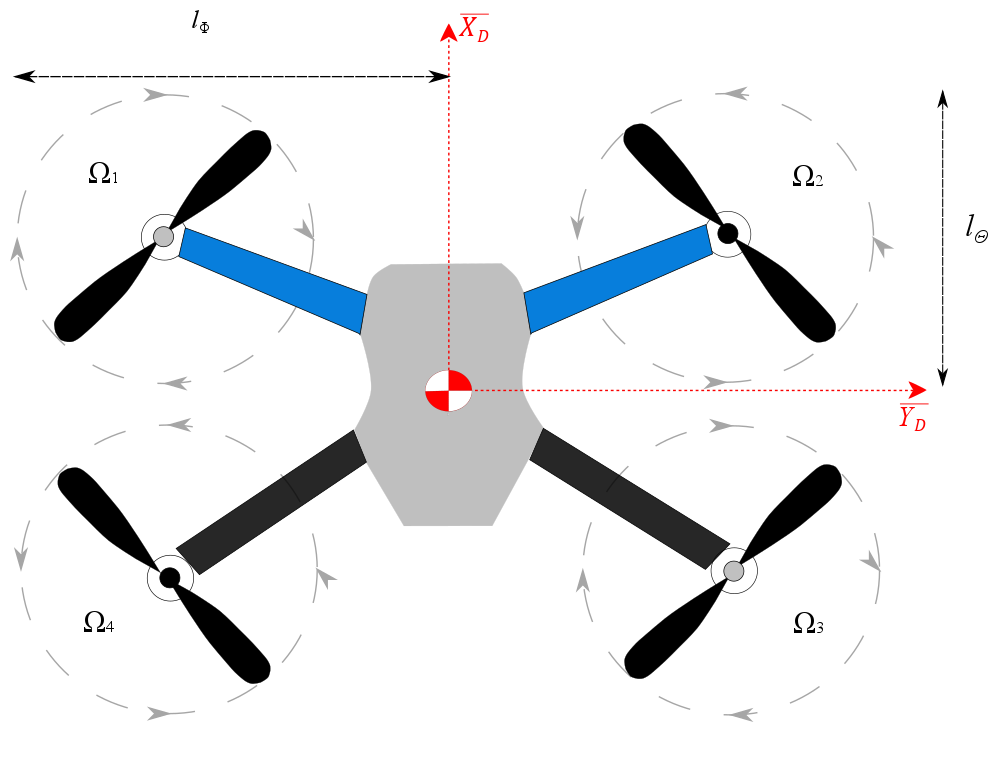
\includegraphics[width=11cm]
{Figures/Iris+QuadcopterDrawing.png}}
\caption{3DR Iris+ quadrotor model.}
\label{iris+}
\end{figure}

The forces exerted on the quadrotor can be determined by using Newton-Euler methodology in summing up the total forces acting on the body. Here, the predominant forces considered are the total thrust, weight, aerodynamic drag, and tether line force. The moving platform force vector $\{X_{D}$,$Y_{D}$,$Z_{D}\}^{T}$ can then be expanded as

\begin{equation}
\begin{Bmatrix}
X_{A}\\Y_{A}\\Z_{A}
\end{Bmatrix}= -T\begin{bmatrix}
0 \\ 0 \\ 1
\end{bmatrix} + \begin{Bmatrix}
X_{A_{D}} \\ Y_{A_{D}} \\ Z_{A_{D}}
\end{Bmatrix}
\label{XYZD}
\end{equation}

In Eq. (\ref{XYZD}), $T$ is the total thrust from the rotors and $\{X_{A_{D}}$,$Y_{A_{D}}$,$Z_{A_{D}}\}^{T}$ is the  total drag on the body. The total drag caused by the thrusting of the motors is a combination of the induced drag and rotor flapping \cite{quadfdnc}. The induced drag acting on the platform is caused by an imbalance in the thrust produced by advancing and retreating blades. This behavior can be modeled as a linear function of multirotor translational velocity in the platform frame. Additionally, drag due to rotor flapping is caused by rotor flexibility, which is function of advance ratio and dependent on the rotor blades and hub design\cite{rotorflap}. Thus, the total drag vector on the platform is expressed as

\begin{equation}
\begin{Bmatrix}
X_{A_{D}} \\ Y_{A_{D}} \\ Z_{A_{D}}
\end{Bmatrix} = -T\begin{Bmatrix}
\left(\frac{A_{1c}}{\sum\limits_{i=1}^4 \Omega_{i}R} + d_{x_{D}}\right)u_{D} - \frac{A_{1s}}{\sum\limits_{i=1}^4 \Omega_{i}R}v_{D} \\
{\frac{A_{1s}}{\sum\limits_{i=1}^4 \Omega_{i}R}}u_{D} + \left(\frac{A_{1c}}{\sum\limits_{i=1}^4 \Omega_{i}R}  + d_{y_{D}}\right)v_{D} \\ 0
\end{Bmatrix}
\label{DAxyz}
\end{equation}
where $d_{x_{D}}$, $d_{y_{D}}$ are the induced drag coefficients and $A_{1s}$,$A_{1c}$ are positive constants that describe the rotor flapping response as a function of advance ratio in Eq. (\ref{advanceratio})

\begin{equation}
\begin{split}
\mu = \frac{\sqrt[]{{u_{D}}^{2} + {v_{D}}^{2}}}{\eta}\\
\eta = {\sum\limits_{i=1}^4 \Omega_{i}R}
\label{advanceratio}
\end{split}
\end{equation}

For quadrotor rotational dynamics, the platform moment vector $\{L_{D}$,$M_{D}$,$N_{D}\}^{T}$ will consider additional aerodynamics created by the rotor torque and also atmospheric wind disturbances. From Kun \textsl{et al.} (2016), the derivation for the angular momentum Newton's Second Law for Rotation results in

\begin{equation}
\{L_{D},M_{D},N_{D}\}^{T}=  \overrightarrow{\Gamma} + \overrightarrow{\tau_{w}} + \overrightarrow{\tau_{A}}
\label{LMNDT}
\end{equation}


For Eq. (\ref{LMNDT}),  $\overrightarrow{\Gamma}$ is the gyroscopic moments, $\overrightarrow{\tau_{w}}$ is wind disturbance torque vector, and $\overrightarrow{\tau_{A}}$ is the aerodynamic torque vector from the rotors. Note that $\overrightarrow{\tau_{w}}=\{\tau_{w_{\phi}},\tau_{w_{\theta}},\tau_w{_{\psi}}\}^{T}$ and $\overrightarrow{\tau_{A}}=\{\tau_{A_{\phi}},\tau_{A_{\theta}},\tau_{A_{\psi}}\}^{T}$ are the expanded forms for the torque vectors. The gyroscopic moments due to the rotors are defined as

\begin{equation}
\overrightarrow{\Gamma} = I_{r}\begin{bmatrix}
p \\ q \\ r
\end{bmatrix}\times\begin{bmatrix}
0 \\ 0\\ \Omega_{r}
\end{bmatrix} = \begin{bmatrix}
I_{r}\Omega_{r}q \\ -I_{r}\Omega_{r}p \\ 0
\end{bmatrix}
\label{Gamma}
\end{equation}

\begin{equation}
\Omega_{r} = \Omega_{1} - \Omega_{2} + \Omega_{3} - \Omega_{4} 
\label{Omegarel}
\end{equation}

where $I_{r}$ is the moment of inertia about the rotor axis and $\Omega_{r}$ is the relative rotor speed. The thrust exerted on the  is made possible due to the counter-rotating blades and allows for easy maneuverability by deviating the rotor angular velocities. It can be simply defined as the sum of the exerted rotor forces $f_{i}$ such that

\begin{equation}
T = \sum\limits_{i=1}^4 f_{i} = f_{1}+f_{2}+f_{3}+f_{4}
\label{Tsimple}
\end{equation}

To induce maneuverability, the Euler angles are deviated as follows 

\begin{equation}
\begin{split}
{\phi}^{+}: \Omega_{2}\Omega_{3} \textgreater \Omega_{1}\Omega_{4}\\
{\theta}^{+}: \Omega_{1}\Omega_{2} \textgreater \Omega_{3}\Omega_{4}\\
{\psi}^{+}: \Omega_{1}\Omega_{3} \textgreater \Omega_{2}\Omega_{4}
\label{ptpplus}
\end{split}
\end{equation}

Based on Eq. (\ref{ptpplus}), the torques are modeled accordingly as 

\begin{equation}
\begin{split}
\tau_{A_{\phi}} = l_{\phi}[(f_{2}+f_{3})-(f_{1}+f_{4})]\\
\tau_{A_{\theta}} = l_{\theta}[(f_{1}+f_{2})-(f_{3}+f_{4})]\\
\tau_{A_{\psi}} = \tau_{1}+\tau_{2}+\tau_{3}+\tau_{4}
\label{tauptp}
\end{split}
\end{equation}


In Eq. (\ref{tauptp}), $l_{\phi}$ and $l_{\psi}$ are the lengths from the rotor axis to the positive platform frame axes for roll and pitch, respectively. Positive yaw torque is achieved by reducing the angular velocity in rotors 2 and 4.  Hoffman \textsl{et al.} (2007) determined that the rotor's angular velocity and thrust varies with angle of attack and is affected by blade flapping and geometry. However, this behavior is complex and difficult to model and is negligible with a low angles of attack and velocities. Kendoul \textsl{et al.} (2007) simplified the thrust model for the rotors approximated as Eq. (\ref{fi}) and similarly for the angular in Eq. (\ref{taui}).

\begin{equation}
f_{i} = k_{t}{\Omega_{i}}^{2}
\label{fi}
\end{equation}

\begin{equation}
\tau_{i} = b{\Omega_{i}}^{2}
\label{taui}
\end{equation}

The constant $b$ in the above equation denote the blade drag factor. Note that these rotor constants are assumed to be constant throughout the flight in order to apply the approximated equations stated. The constants can be summarized as a factor that results from the momentum theory of the blade element\cite{swingload}. Therefore 

\begin{equation}
k_{t} = C_{T}\frac{4\rho {R}^{4}}{{\pi}^{2}}
\label{kt}
\end{equation}

\begin{equation}
b = C_{\tau}\frac{4\rho {R}^{5}}{{\pi}^{3}}
\label{b}
\end{equation}

In Eqs. (\ref{kt}-\ref{b}), $\rho$ is the air density, $C_{T}$ is the thrust factor, and $C_{Q}$ is the momentum factor. A summarized form for Eq. (\ref{tauptp}) can be seen as

\begin{equation}
\begin{Bmatrix}
\tau_{A_{\phi}}\\ \tau_{A_{\theta}} \\ \tau_{A_{\psi}}
\end{Bmatrix} = \begin{bmatrix}
-k_{t}l_{\phi} & k_{t}l_{\phi} & -k_{t}l_{\phi} & k_{t}l_{\phi}\\
k_{t}l_{\theta} & -k_{t}l_{\theta} & k_{t}l_{\theta} & -k_{t}l_{\theta}\\
b & -b & b & -b
\end{bmatrix}\begin{Bmatrix}
{\Omega_{1}}^2\\ {\Omega_{2}}^2\\ {\Omega_{3}}^2\\ {\Omega_{4}}^2
\end{Bmatrix}
\label{tauptpfinal}
\end{equation}

\subsubsection{Spacecraft Aerodynamics}

The aerodynamic force is computed using aerodynamic coefficients and
dynamic pressure where $\vec{V}$ is the velocity of the satellite and
$V$ is the magnitude of the velocity vector. Furthermore, $S$ is the
surface area of the satellite and $C_D$ is the drag coefficient. The
torque on the satellite is then given by the cross product between the
aerodynamic force and a distance vector representing the distance
between the center of mass and the center of pressure
$\vec{r}_{CP-CG}$.
\begin{equation}
  \vec{F}_A = \frac{1}{2}\rho V\vec{V}S C_D
\end{equation}
\begin{equation}
    \vec{M}_A = -{\bf S}\left(\vec{F}_A\right)\vec{r}_{CP-CG}
\end{equation}